\documentclass[12pt]{article}
\usepackage[letterpaper,margin=0.65in,top=0.8in,headheight=16pt,headsep=17pt,footskip=24pt]{geometry}
\usepackage[T1]{fontenc}
\usepackage{lmodern}
\renewcommand{\familydefault}{\sfdefault}
\usepackage{tikz}
\usetikzlibrary{arrows.meta}
\usepackage{fancyhdr}
\pagestyle{fancy}\fancyhf{}
\renewcommand{\headrulewidth}{0.35pt}
\fancyfoot[C]{\fontsize{9}{11}\selectfont Bellingham Math Circle / Week 16 / W16-RV-draft / \thepage}
\setlength{\parindent}{0pt}\setlength{\parskip}{9pt}
\newcommand{\header}[1]{\fancyhead[C]{\fontsize{11.5}{14}\selectfont Week 16 / Three-color meshes / #1}}
\newcommand{\problem}[2]{\textbf{Problem #1:} #2\par}
\newcommand{\blankdot}[2]{\draw[fill=white,line width=0.8pt] (#1,#2) circle[radius=0.14in];}
\newcommand{\letterdot}[3]{\draw[fill=white,line width=0.8pt] (#1,#2) circle[radius=0.14in];\node[font=\large] at (#1,#2) {#3};}
\begin{document}\fontsize{14}{17.5}\selectfont
\header{Grades K--1 and up}
Keep the corner letters. A dot on a side uses one of that side's corner letters.
Inside, use R, B, Y or G. Count only triangles with no lines inside them.

\problem{1}{Which middle letters leave no small triangle with R, B and Y? Find every choice.}
\begin{center}
\begin{tikzpicture}[x=1.35in,y=1.35in]
\draw[line width=0.6pt] (0,0)--(3,0)--(1.5,2.59807621)--cycle;
\draw[line width=0.6pt] (0,0)--(1.5,0.86602540)--(3,0);
\draw[line width=0.6pt] (1.5,0.86602540)--(1.5,2.59807621);
\letterdot{0}{0}{R}\letterdot{3}{0}{B}\letterdot{1.5}{2.59807621}{Y}
\blankdot{1.5}{0.86602540}
\end{tikzpicture}
\end{center}
\vspace{0.35in}
\rule{\linewidth}{0.35pt}\par\vspace{0.45in}
\rule{\linewidth}{0.35pt}\par\vspace{0.45in}
\rule{\linewidth}{0.35pt}

\newpage\header{Grades 2--3 and up}
\problem{2}{Fill the blank dots so no small triangle has R, B and Y. Among those fillings, how few small triangles can have three different letters?}
\begin{center}
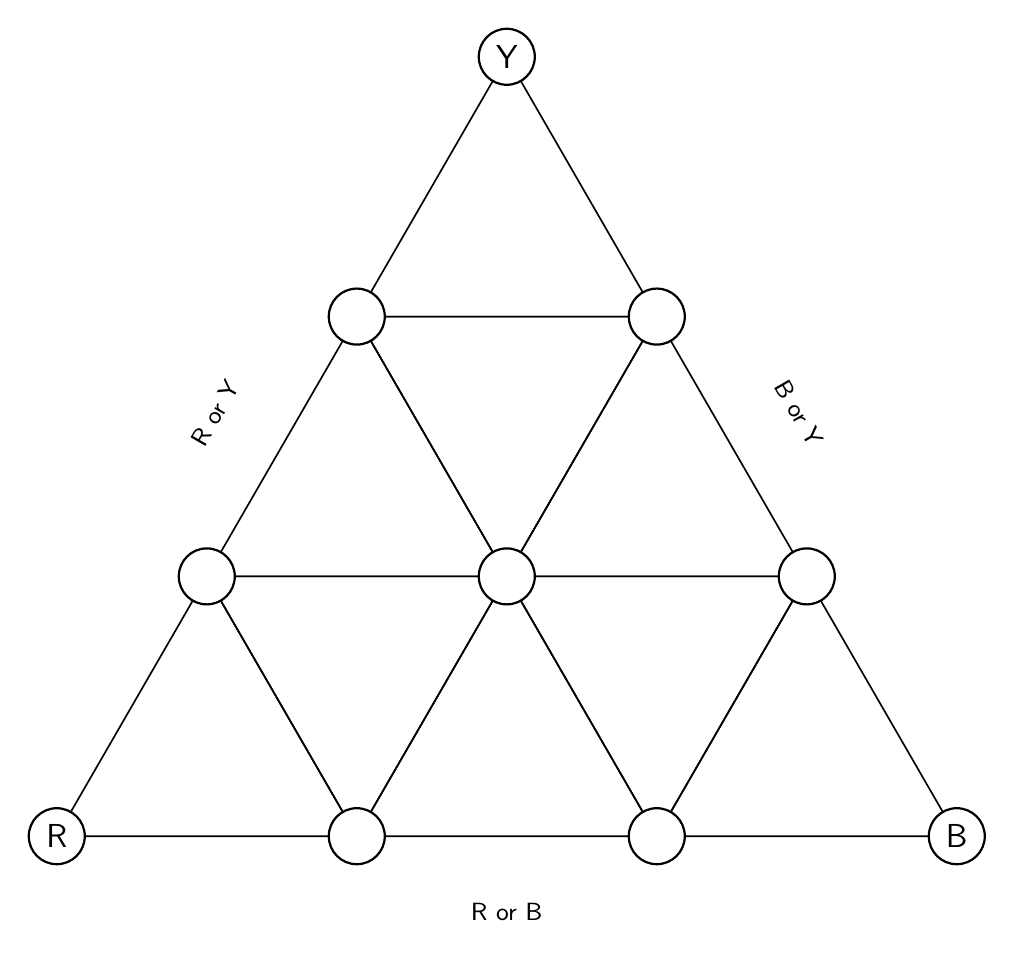
\begin{tikzpicture}[x=1.5in,y=1.5in]
\draw[line width=0.6pt] (0.00000000,0.00000000)--(1.00000000,0.00000000)--(0.50000000,0.86602540)--cycle;
\draw[line width=0.6pt] (1.00000000,0.00000000)--(1.50000000,0.86602540)--(0.50000000,0.86602540)--cycle;
\draw[line width=0.6pt] (1.00000000,0.00000000)--(2.00000000,0.00000000)--(1.50000000,0.86602540)--cycle;
\draw[line width=0.6pt] (2.00000000,0.00000000)--(2.50000000,0.86602540)--(1.50000000,0.86602540)--cycle;
\draw[line width=0.6pt] (2.00000000,0.00000000)--(3.00000000,0.00000000)--(2.50000000,0.86602540)--cycle;
\draw[line width=0.6pt] (0.50000000,0.86602540)--(1.50000000,0.86602540)--(1.00000000,1.73205081)--cycle;
\draw[line width=0.6pt] (1.50000000,0.86602540)--(2.00000000,1.73205081)--(1.00000000,1.73205081)--cycle;
\draw[line width=0.6pt] (1.50000000,0.86602540)--(2.50000000,0.86602540)--(2.00000000,1.73205081)--cycle;
\draw[line width=0.6pt] (1.00000000,1.73205081)--(2.00000000,1.73205081)--(1.50000000,2.59807621)--cycle;
\letterdot{0.00000000}{0.00000000}{R}
\blankdot{1.00000000}{0.00000000}
\blankdot{2.00000000}{0.00000000}
\letterdot{3.00000000}{0.00000000}{B}
\blankdot{0.50000000}{0.86602540}
\blankdot{1.50000000}{0.86602540}
\blankdot{2.50000000}{0.86602540}
\blankdot{1.00000000}{1.73205081}
\blankdot{2.00000000}{1.73205081}
\letterdot{1.50000000}{2.59807621}{Y}
\node[font=\small,anchor=north] at (1.5,-0.19) {R or B};
\node[font=\small,rotate=60,anchor=south] at (0.58,1.38) {R or Y};
\node[font=\small,rotate=-60,anchor=south] at (2.42,1.38) {B or Y};
\end{tikzpicture}
\end{center}
\vspace{0.20in}
\rule{\linewidth}{0.35pt}\par\vspace{0.55in}
\rule{\linewidth}{0.35pt}\par\vspace{0.55in}
\rule{\linewidth}{0.35pt}

\newpage\header{Grades 2--3 and up}
Use only R, B and Y. A rainbow triangle has R, B and Y and no lines inside.

\problem{3}{Label the corners, giving matching corners the same letter on the two squares in each row. Can switching the diagonal change the number of rainbow triangles? Can it change whether that number is even or odd? Find a rule from the outside letters.}
\begin{center}
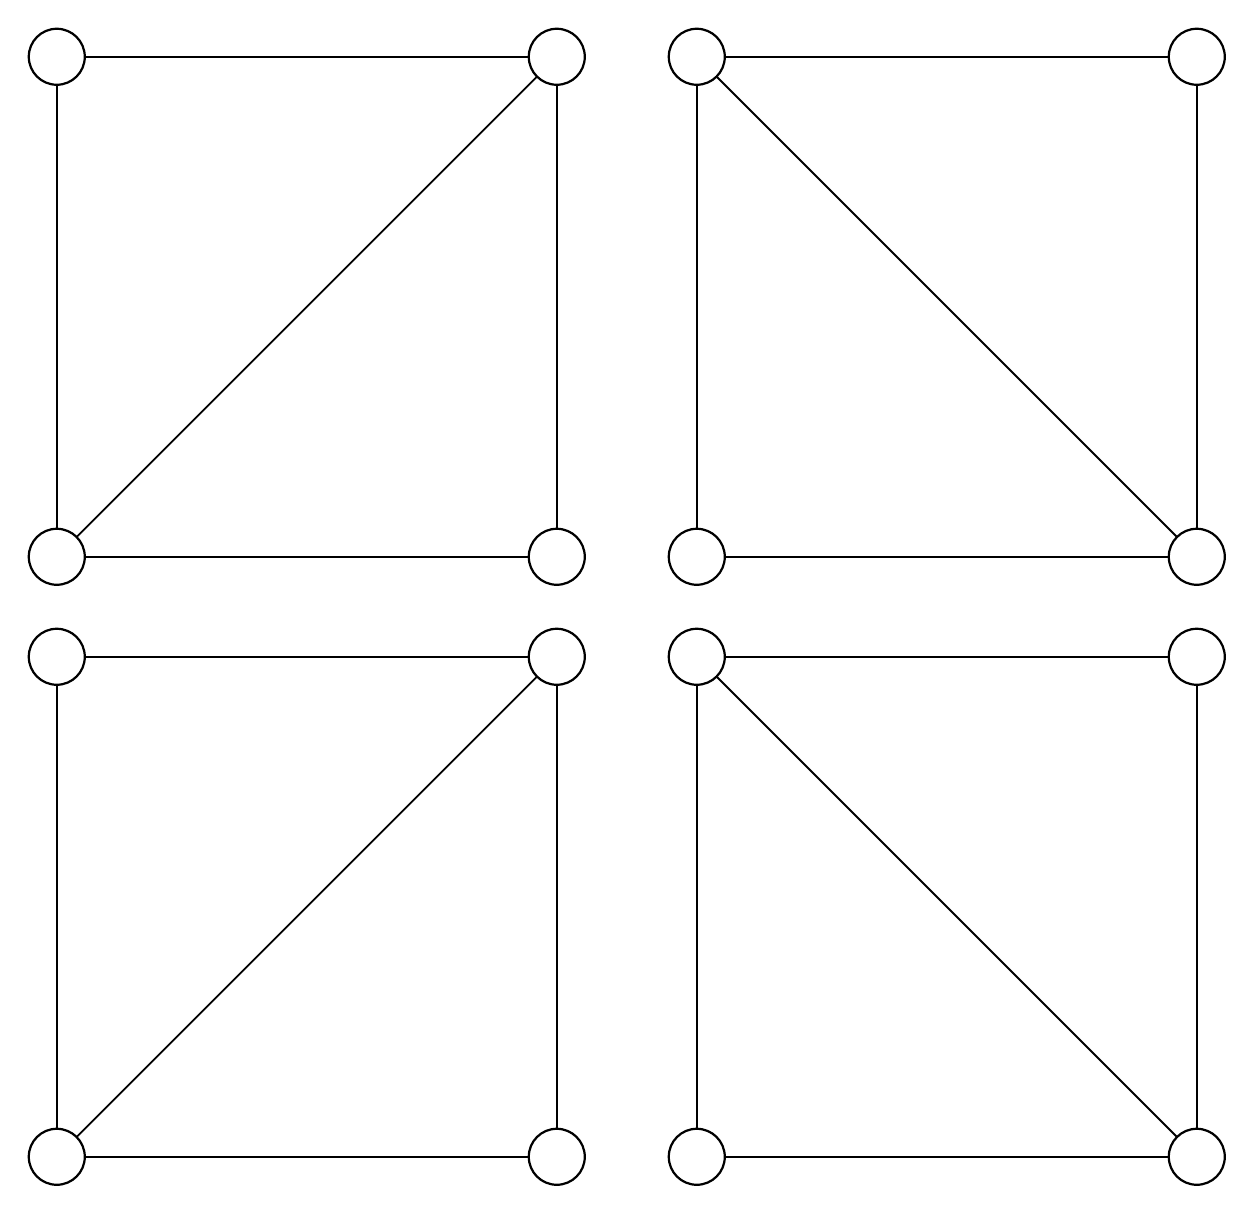
\begin{tikzpicture}[x=1in,y=1in]
\begin{scope}[shift={(0,3.0)}]
\draw[line width=0.65pt] (0,0) rectangle (2.5,2.5);
\draw[line width=0.65pt] (0,0)--(2.5,2.5);
\blankdot{0}{0}
\blankdot{2.5}{0}
\blankdot{2.5}{2.5}
\blankdot{0}{2.5}
\end{scope}
\begin{scope}[shift={(3.2,3.0)}]
\draw[line width=0.65pt] (0,0) rectangle (2.5,2.5);
\draw[line width=0.65pt] (0,2.5)--(2.5,0);
\blankdot{0}{0}
\blankdot{2.5}{0}
\blankdot{2.5}{2.5}
\blankdot{0}{2.5}
\end{scope}
\begin{scope}[shift={(0,0)}]
\draw[line width=0.65pt] (0,0) rectangle (2.5,2.5);
\draw[line width=0.65pt] (0,0)--(2.5,2.5);
\blankdot{0}{0}
\blankdot{2.5}{0}
\blankdot{2.5}{2.5}
\blankdot{0}{2.5}
\end{scope}
\begin{scope}[shift={(3.2,0)}]
\draw[line width=0.65pt] (0,0) rectangle (2.5,2.5);
\draw[line width=0.65pt] (0,2.5)--(2.5,0);
\blankdot{0}{0}
\blankdot{2.5}{0}
\blankdot{2.5}{2.5}
\blankdot{0}{2.5}
\end{scope}
\end{tikzpicture}
\end{center}
\vspace{0.15in}\rule{\linewidth}{0.35pt}

\newpage\header{Grades 4--5}
Use only R, B and Y. Keep the corner letters and side choices shown.
A rainbow triangle has R, B and Y and no lines inside. Read it counterclockwise,
starting at R. Mark it $+$ or $-$ as shown.
\begin{center}
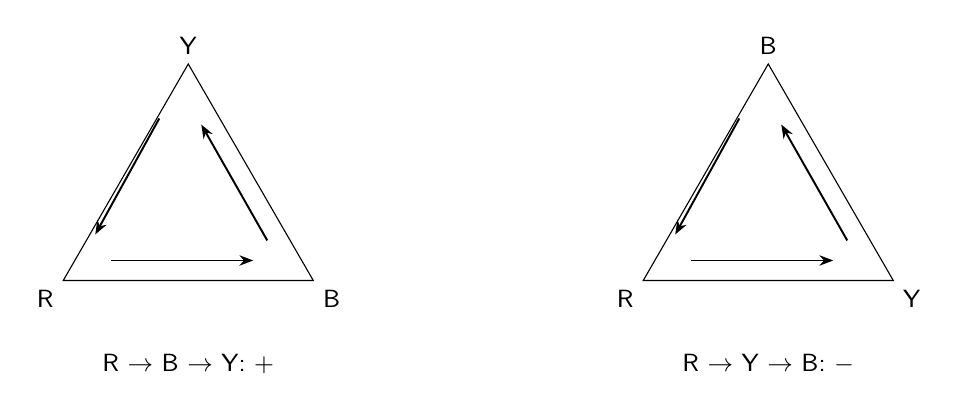
\begin{tikzpicture}[x=1in,y=1in,font=\small]
\begin{scope}
\draw (0,0)--(1.25,0)--(0.625,1.08253175)--cycle;
\node[anchor=north east] at (0,0) {R};\node[anchor=north west] at (1.25,0) {B};\node[anchor=south] at (0.625,1.08253175) {Y};
\draw[-{Stealth[length=5pt]},line width=0.7pt] (0.24,0.10)--(0.95,0.10);
\draw[-{Stealth[length=5pt]},line width=0.7pt] (1.02,0.20)--(0.69,0.78);
\draw[-{Stealth[length=5pt]},line width=0.7pt] (0.48,0.81)--(0.16,0.23);
\node[anchor=north] at (0.625,-0.32) {R $\to$ B $\to$ Y: $+$};
\end{scope}
\begin{scope}[shift={(2.9,0)}]
\draw (0,0)--(1.25,0)--(0.625,1.08253175)--cycle;
\node[anchor=north east] at (0,0) {R};\node[anchor=north west] at (1.25,0) {Y};\node[anchor=south] at (0.625,1.08253175) {B};
\draw[-{Stealth[length=5pt]},line width=0.7pt] (0.24,0.10)--(0.95,0.10);
\draw[-{Stealth[length=5pt]},line width=0.7pt] (1.02,0.20)--(0.69,0.78);
\draw[-{Stealth[length=5pt]},line width=0.7pt] (0.48,0.81)--(0.16,0.23);
\node[anchor=north] at (0.625,-0.32) {R $\to$ Y $\to$ B: $-$};
\end{scope}
\end{tikzpicture}
\end{center}
\problem{4}{Fill the blank dots and mark the rainbow triangles. What can change between fillings, and what stays the same about the two totals?}
\begin{center}
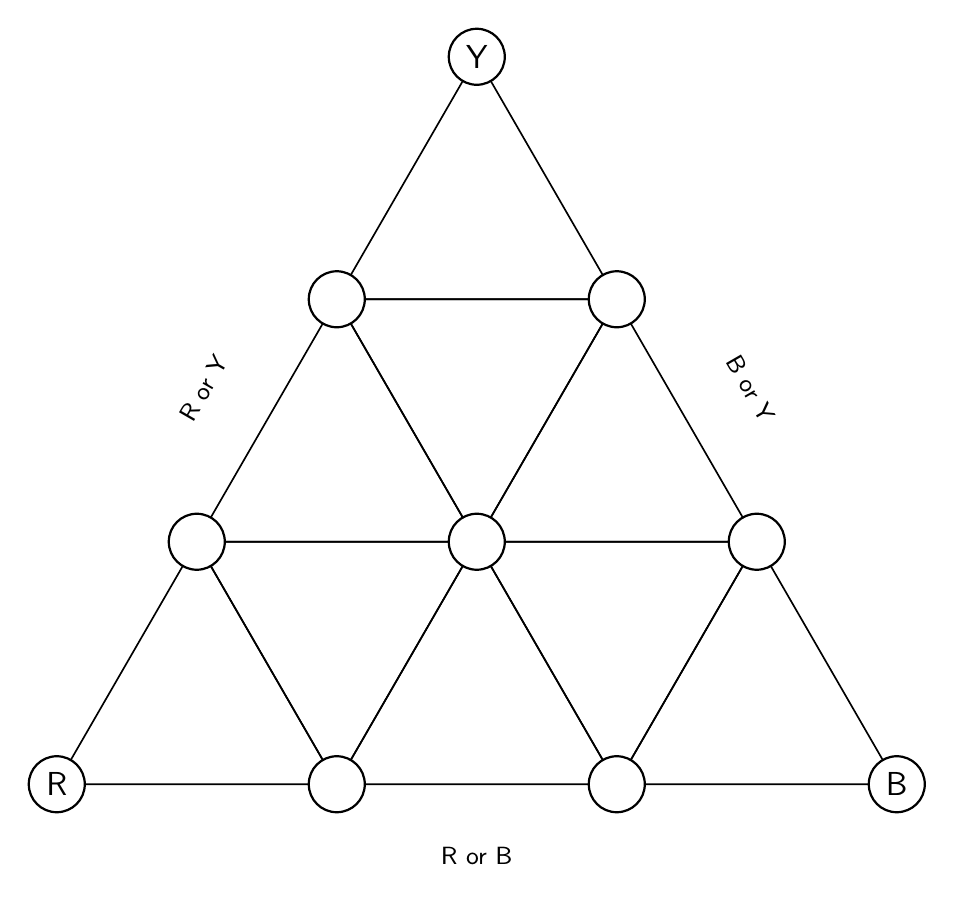
\begin{tikzpicture}[x=1.4in,y=1.4in]
\draw[line width=0.6pt] (0.00000000,0.00000000)--(1.00000000,0.00000000)--(0.50000000,0.86602540)--cycle;
\draw[line width=0.6pt] (1.00000000,0.00000000)--(1.50000000,0.86602540)--(0.50000000,0.86602540)--cycle;
\draw[line width=0.6pt] (1.00000000,0.00000000)--(2.00000000,0.00000000)--(1.50000000,0.86602540)--cycle;
\draw[line width=0.6pt] (2.00000000,0.00000000)--(2.50000000,0.86602540)--(1.50000000,0.86602540)--cycle;
\draw[line width=0.6pt] (2.00000000,0.00000000)--(3.00000000,0.00000000)--(2.50000000,0.86602540)--cycle;
\draw[line width=0.6pt] (0.50000000,0.86602540)--(1.50000000,0.86602540)--(1.00000000,1.73205081)--cycle;
\draw[line width=0.6pt] (1.50000000,0.86602540)--(2.00000000,1.73205081)--(1.00000000,1.73205081)--cycle;
\draw[line width=0.6pt] (1.50000000,0.86602540)--(2.50000000,0.86602540)--(2.00000000,1.73205081)--cycle;
\draw[line width=0.6pt] (1.00000000,1.73205081)--(2.00000000,1.73205081)--(1.50000000,2.59807621)--cycle;
\letterdot{0.00000000}{0.00000000}{R}
\blankdot{1.00000000}{0.00000000}
\blankdot{2.00000000}{0.00000000}
\letterdot{3.00000000}{0.00000000}{B}
\blankdot{0.50000000}{0.86602540}
\blankdot{1.50000000}{0.86602540}
\blankdot{2.50000000}{0.86602540}
\blankdot{1.00000000}{1.73205081}
\blankdot{2.00000000}{1.73205081}
\letterdot{1.50000000}{2.59807621}{Y}
\node[font=\small,anchor=north] at (1.5,-0.19) {R or B};
\node[font=\small,rotate=60,anchor=south] at (0.58,1.38) {R or Y};
\node[font=\small,rotate=-60,anchor=south] at (2.42,1.38) {B or Y};
\end{tikzpicture}
\end{center}
\begin{center}
\begin{tabular}{p{2in}p{2in}}
$+$ total: \hrulefill & $-$ total: \hrulefill \\[13pt]
$+$ total: \hrulefill & $-$ total: \hrulefill \\[13pt]
$+$ total: \hrulefill & $-$ total: \hrulefill
\end{tabular}
\end{center}
\end{document}
